
\section{Software} \label{sec:software}
In diesem Kapitel wird die Umsetzung der Berechnung (Kapitel 3 \ref{sec:umsetzung}) und der anderen Anforderungen an die Software in Java dokumentiert. Die programmiertechnischen Grundlagen sind in Kapitel 2 \ref{sec:grundlagen} beschrieben.


\subsection{Übersicht} \label{subsec:uebersicht}
%TODO Einfügen Bild GUI

Die Software ist nach dem MVC Framework (TODO:Verweis) aufgebaut. Das Klassendiagramm der Software befindet sich im Anhang (TODO: Verweis). Die View ist für die Darstellung der Daten und die Verarbeitung der Benutzereingaben zuständig. Zur View gehören die Panels: InputPanel (1), FiltertablePanel (2), ButtonPanel (3), Menubar (4) und PlotPanel (5). In diesem Abschnitt werden die Panels dokumentiert Diese bilden zusammen die Benutzeroberfläche, die in der Abbildung (TODO verweis) ersichtlich ist. Im Klassendiagramm (TODO Verweis Anhang) sind alle Klassen die zur View gehören, mit der Farbe (TODO: Farbe) markiert.

%Diese Infos gehören auch noch rein
%Die Oben abgebildete Benutzerfläche ist die Maske, welche sich beim aufstauten der Software auf dem Bildschirm präsentiert. Wie die  meisten gängigen Applikationen verfügt die GUI eine am oberen Rand platzierten Menubar, um Dateien zu verwalten sowie Hilfestellung zu bieten. Im Zentrum ist im oberen Bereich das Plotpanel platziert, welches die Simulation sowohl im Gleichtakt (CM), als auch im Gegentakt (DM) als grafische Kurve darstellt. Gleich unterhalb befindet sich das Inputpanal, es ermöglicht mittels den Textfeldern eine  effiziente Eingabe der  Parameter. Mittels den Sleidern können die Parameter prozentual angepasst werden. Die Filtertabelle links dient zur Verwaltung der Filterprofilen.


%TODO Model und Controller Anteasern(Wie dieses Beispiel)
%Das Model hat eine SignalQuelle, eine Verzögerung und ein LMSFilter. Die SignalQuelle erzeugt das mit einem Störton gestörte Nutzsignal und erbt zu diesem Zwecke von der Klasse Thread. Sie ruft in regelmässigen Abständen via SignalListener die Methode processSignal(signal : double[]) mit einem Block von digitalen Signalwerten auf. Die Signalwerte werden dann, zur Estimation des Störtons durch die Verzögerung und durch das LMSFilter geschickt und letzteres mittels Fehlersignal adaptiert. 

%Der Controller delegiert im Wesentlichen die Aufgaben ans Model, welches wiederum via Observer - Observable Entwurfsmuster zum Aufdatieren der View führt.


\subsection{Model} \label{subsec:Model}

to be done => Beispiel Anschauen von Hr Gut
%TODO Methoden der Klasse Model beschreiben



\subsection{View} \label{subsec:view}
Die View ist als GridBagLayout organisiert und enthält die im Kapitel \ref{subsec:uebersicht} erwähnten Panels.
\bigskip

\paragraph{Inputpanel} \label{par:inputpanel}
Das InputPanel hat den Controller und ist im GridBagLayout organisiert. Das Panel wird in mehreren Subpanels unterteilt. Diese sind in der Abbildung  \ref{fig:subpanels} abgebildet. 

\begin{figure}[H]
	\centering
	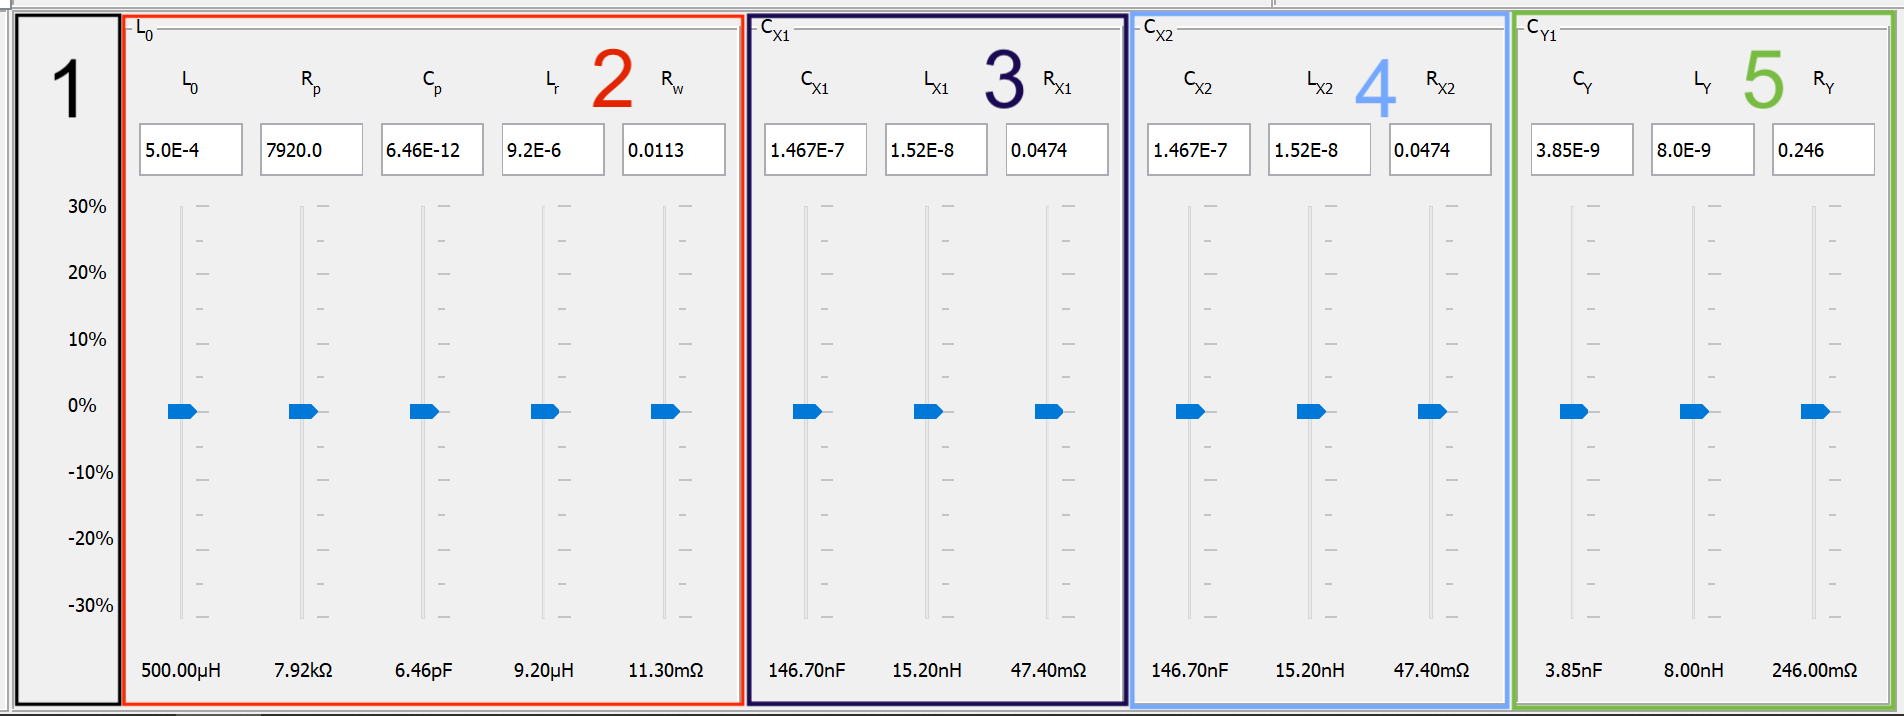
\includegraphics[width=13cm]{SubPanels.png}
	\caption{InputSubPanels}
	\label{fig:subpanels}
\end{figure} 

Das InformationPanel(1) ist im Null-Layout organisiert. Es werden die Prozentzahlen der Schieberegler dargestellt. Diese sind an einer festen Position, da die Grösse des Inputpanels nicht verändert werden kann. Die weiteren Subpanels (2-5) sind im GridBagLayout organisiert. In diesen Panels befinden sich die Komponenten, der modellierten realen Bauteile. Jede Komponente besitzt ein Textfeld, einen Slider und ein Label. Im Textfeld kann der Benutzer seine Werte für die Komponente eintragen. Beim Aufstarten des Programmes wird das Feld mit einem Standardwert, der vom Auftragdokument übernommen wurde, geladen. Mit der Klasse JEngineerField werden die Eingaben geprüft. Es ist nur möglich Zahlen einzugeben. Grosse und kleine Zahlen können zur Vereinfachung in wissenschaftlicher Schreibweise (18e-12) oder in Einheiten-Schreibweise (18p) eingetragen werden. Die Ausgabe ist als Einheiten-Schreibweise vordefiniert. Mit einem Rechtsklick auf das Textfeld ist es möglich die Schreibweise der Eingabe und Ausgabe individuell zu verändern.
Mit dem Schieberegler wird der im Textfeld eingegebener Wert um $\pm$ 30\% verändert und im Label als effektiver Wert ausgegeben. Das Textfeld besitzt einen ActionListener und der Slider einen changeListener. Bei einem Ereignis wird die dazugehörige Methode im Controller  aufgerufen.
\bigskip

\paragraph{Filtertablepanel} \label{par:filterpanel}
Das Filtertablepanel hat den Controller und ist im GridBagLayout organisiert. Es enthält eine Tabelle, in der die Parameterwerte hinterlegt und zu dem entsprechenden Filter zugeordnet werden. Jeder Filter in der Tabelle besitzt eine Checkbox, um den Filter zu aktivieren, und ein Textfeld, um den Filter  zu benennen. Die Tabelle hat einen TableModelListener und einen ListSelectionListener. Bei einem Ereignis wird die dazugehörige Methode im Controller  aufgerufen.
\bigskip

\paragraph{Buttonpanel} \label{par:buttonpanel}
Das ButtonPanel hat den Controller und ist im Null-Layout organisiert. Es enthält die vier Buttons und zwei dazugehörige Labels. Mit diesen kann die Filtertabelle verwaltet und die Speicherverwaltung aufgerufen werden. Jeder Button hat einen ActionListener. Bei einem Ereignis wird die dazugehörige Methode im Controller  aufgerufen.
\bigskip

\paragraph{Plotpanel} \label{par:plotpanel}
Das PlotPanel ist im BorderLayout organisiert. Mit Hilfe des Package JfreeChart (TODO: verweis) wird die Einfügedämpfung des EMI-Filters in einem Plot dargestellt. Das Package übernimmt viele Funktionen wie das Zoomen des Plots oder das Ändern der Darstellung. Löst der Observer ein Erreignis aus, werden die Daten vom Model geholt und geplottet.
\bigskip

\newpage

\paragraph{Menubar} \label{par:menu}
Das Menubar hat den Controller und ist im Null-Layout organisiert. Es besitzt die Menus File, in dem die Speicherverwaltung aufgerufen werden kann, Circuit, in dem die Schaltungen, von denen die Berechnungen ausgehen angezeigt werden und About, in dem Informationen über das Programm hinterlegt sind. Die Menüs haben einen ActionListener. Bei einem Ereignis wird die dazugehörige Methode im Controller  aufgerufen.



\subsection{Controller} \label{subsec:controller}

Der Controller dient als Schnittstelle zwischen dem Model und der View. Dabei werden die von View aufgerufenen Funktionen an das Model weitergeleitet. Diese Werte, die das Model Berechnet hat, werden anschliessend wieder an den Controller gesendet und zurück zur View geleitet. Der Controller besteht aus 9 Methoden, wobei eine der Konstruktor ist. Von diesen Methoden wird das Model nur von den beiden Methoden calculateInsertionloss() und deleteRowInCalculationData() aufgerufen. Die Methode calculateInsertionloss() ist dafür zuständig den Insertionloss für die Schaltungen, mit den in der GUI  eingestellt Parametern, zu berechnen.  


\subsection{Trace} \label{trace}
Um den Ablauf innerhalb der Software nachvollziehen zu können wird nachfolgend die Sogenannte "Trace" beim Aufstarten der Software und beim Auslösen eines Ereignisses aufgezeigt. Die "Trace" wird innerhalb der Software mithilfe der Klasse traceV4 in die Konsole ausgegeben.



